\chapter{Je plaats op een ronde Aarde}

Wanneer je opzoekt waar je bent of waar je naar toe gaat, kijk je vrijwel altijd op een kaart. Of je dit nu doet met een papieren kaart, een informatiebord langs de weg of met een app op je telefoon, \'e\'en ding hebben ze gemeen: De kaart is plat. Maar de Aarde is allesbehalve plat en het vertalen van de ronde aarde naar een platte kaart is niet eenvoudig.

In dit hoofdstuk ga je leren wat er bij komt kijken om te navigeren op een ronde wereld en hoe het toch, met enige beperkingen, mogelijk is om platte kaarten te gebruiken voor een ronde Aarde.

\section{Co\"ordinaten op een boloppervlak}

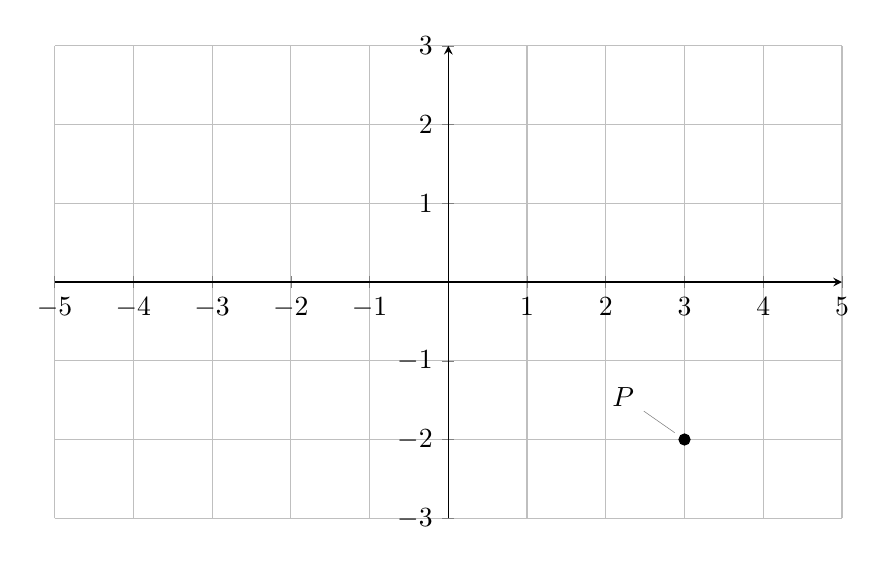
\begin{tikzpicture}
    \begin{axis}[axis lines = middle, grid = both, 
                 xmin = -5, xmax = 5, ymin = -3, ymax = 3,
                 x = 1cm, y = 1cm,
                 xtick = {-5, -4, -3, -2, -1, 0, 1, 2, 3, 4,5},
                 ytick = {-3, -2, -1, 0, 1, 2, 3}]
        \addplot[mark=*] coordinates {(3,-2)} node[pin=150:{$P$}]{} ;
    \end{axis}
	\label{fig_carthesisch}
\end{tikzpicture}

Hierboven zie je een voorbeeld van een plat rooster. Misschien heb je dit al eerder gezien tijdens de wiskundeles. Zo'n rooster zou je kunnen gebruiken om over een kaart heen te leggen. Langs de \textit{x}-as en \textit{y}-as staan getallen waarmee we de co\"ordinaten van punten in het rooster kunnen bepalen. Je kunt het punt met \textit{x} = 2 en \textit{y} = 3 vinden door op de \textit{x}-as de waarde 2 op te zoeken en op de \textit{y}-as de waarde 3. Het gezochte punt is vervolgens te vinden op de plek waar de 2 lijnen vanuit de gevonden punten op de assen elkaar snijden. Een korte notatie voor de co\"ordinaten van dit punt is $(2, 3)$.

\begin{opgave}
	\begin{subopgave}
		Waar ligt het punt (4, 1) in bovenstaand rooster?
		\begin{antwoord}		
			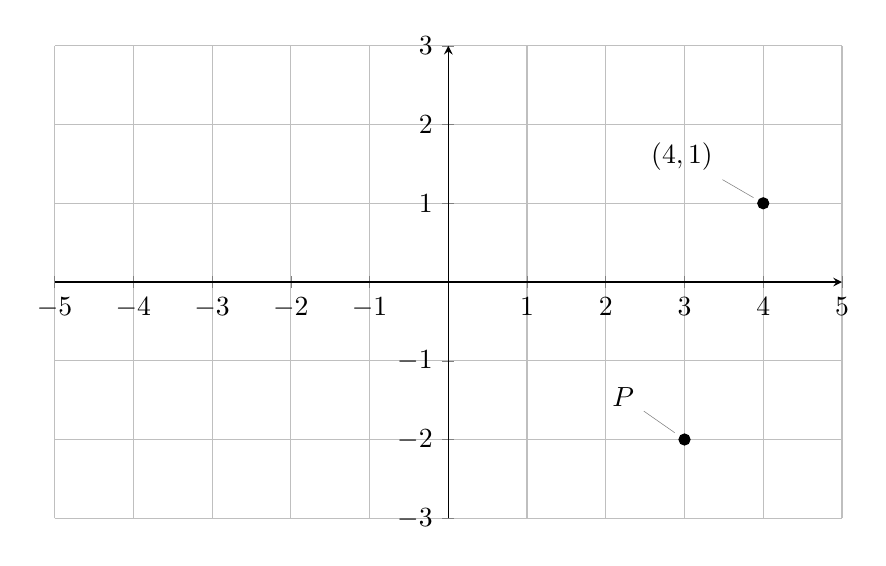
\begin{tikzpicture}
			    \begin{axis}[axis lines = middle, grid = both, 
		                 xmin = -5, xmax = 5, ymin = -3, ymax = 3,
                		 x = 1cm, y = 1cm,
        		         xtick = {-5, -4, -3, -2, -1, 0, 1, 2, 3, 4,5},
		                 ytick = {-3, -2, -1, 0, 1, 2, 3}]
			        \addplot[mark=*] coordinates {(3,-2)} node[pin=150:{$P$}]{} ;
			        \addplot[mark=*] coordinates {(4,1)} node[pin=150:{$(4, 1)$}]{} ;
			    \end{axis}
			\end{tikzpicture}
		\end{antwoord}
	\end{subopgave}
	\begin{subopgave}
		Wat zijn de co\"ordinaten van het in het bovenstaand rooster aangegeven punt P?
		\begin{antwoord}
			$(3, -2)$
		\end{antwoord}
	\end{subopgave}
\end{opgave}

Omdat de Aarde een bol is\footnote{Precies gezegd is de Aarde geen perfecte bol, maar een afgeplatte ellipso\"ide. De straal van de Aarde bij de evenaar is iets groter dan bij de polen. In dit onderzoeksprogramma gaan we echter uit van een bol.} hebben we voor plaatsen op het aardoppervlak een ander systeem van co\"ordinaten nodig, de zogenaamde bolco\"ordinaten. In plaats van \textit{x} en \textit{y} waardes, praten we over lengtegraden en breedtegraden.

\begin{figure}[h]
	\centering
	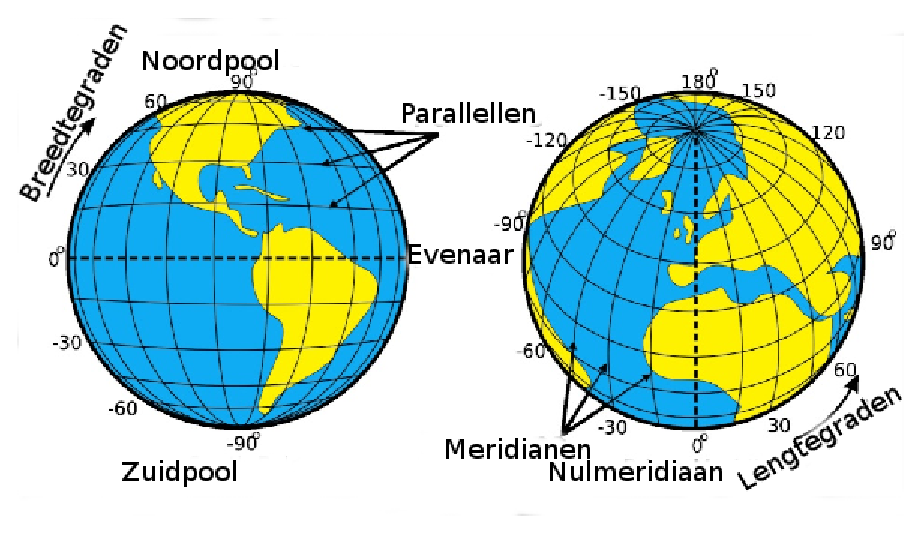
\includegraphics[width=15cm]{Parallels-and-Meridians-nl.eps}
	\caption{parallellen en meridianen}
	\label{fig_par_mer}
\end{figure}

De lengtegraad wordt gemeten langs de horizontale lijnen in bovenstaande figuur, terwijl de breedtegraad gemeten wordt langs de verticale lijnen. Lijnen met constante lengtegraad worden ook wel meridianen genoemd. Lijnen met constante breedtegraad heten parallellen. De belangrijkste meridiaan is de nul-meridiaan die door de Engelse plaats Greenwich loopt. Lengtegraden worden uitgedrukt ten opzichte van deze nul-meridiaan. Bij de parallellen is er een vergelijkbare situatie: De nul-parallel is beter bekend als de evenaar.

Lengte- en breedtegraden worden uitgedrukt in graden, zoals de naam al impliceert. Lengtegraden lopen van $-180\degree$ tot $+180\degree$ en breedtegraden van $-90\degree$ tot $+90\degree$. Meestal worden in plaats van min- en plus-tekens echter de windrichtingen gebruikt. Zo wordt een breedtegraad van $40\degree$ boven de evenaar geschreven als $40\degree N$ (N van Noord) en een lengtegraad van $15\degree$ ten oosten van de nul-meridiaan wordt geschreven als $15\degree E$ (E van East, oftewel Oost).

\begin{opgave}
	Lengtegraden hebben een totaal bereik van $360\degree$, terwijl breedtegraden slechts een bereik van $180\degree$ hebben. Waarom is het niet nodig dat breedtegraden ook een bereik van $360\degree$ hebben?
	\begin{antwoord}
		Neem een cirkel, deze stelt de $360\degree$ aan lengtegraden op de evenaar voor. Roteer de cirkel nu om een as die door het midden van deze cirkel loopt. Bij het roteren vormt zich een boloppervlak. Merk op dat de cirkel slechts $180\degree$ geroteerd hoeft te worden om een volledige bol te maken, niet $360\degree$. Als de breedtegraden ook een bereik van $360\degree$ zouden hebben, dan zou ieder punt op Aarde twee sets co\"ordinaten hebben.
	\end{antwoord}
\end{opgave}

\begin{opgave}
	\begin{subopgave}
		De straal van de Aarde is ongeveer 6400~km. Wat is de omtrek van de Aarde?
		\begin{antwoord}
			12800 km * $\pi$ = 40200 km
		\end{antwoord}			
	\end{subopgave}
	\begin{subopgave}
		Hoe ver moet je over de evenaar reizen om de lengtegraad van je positie met $1\degree$ te veranderen?
		\begin{antwoord}
			1/360 * 40200 km = 112 km
		\end{antwoord}
	\end{subopgave}
	\begin{subopgave}
		De parallel die door Heino loopt heeft een straal van ongeveer 3900~km. Hoe groot is de omtrek van deze parallel?
		\begin{antwoord}
			24500 km
		\end{antwoord}
	\end{subopgave}
	\begin{subopgave}
		Als je vanuit Heino $1\degree$ lengtegraad verplaatst, welke afstand leg je dan af?
		\begin{antwoord}
			$\frac{24500}{360} = 68$~km
		\end{antwoord}
	\end{subopgave}
\end{opgave}

Omdat het makkelijker is om het aardoppervlak plat weer te geven, hebben we een manier nodig om het bolvormige oppervlak op een plat rooster over te zetten. Een voor de hand liggende manier is om de boel zo af te beelden dat meridianen verticale lijnen worden op het platte rooster en parallellen horizontale lijnen.

\begin{figure}[h]
	\centering
	\includegraphics[width=15cm]{Equirectangular_projection_SW.eps}
	\caption{De aarde afgebeeld op een plat vlak}
	\label{fig_equirect}
\end{figure}

\begin{opgave}
	Op het aardoppervlak staan parallellen en meridianen loodrecht op elkaar. Blijft dat nog steeds zo als we het aardoppervlak op bovenstaande manier afbeelden?
	\begin{antwoord}
		Ja.
	\end{antwoord}
\end{opgave}

\begin{opgave}[\vinger]
	\begin{subopgave}
		In een plat rooster is de afstand tussen twee verticale lijnen overal hetzelfde. Is dit ook zo met meridianen op een boloppervlak?
		\begin{hint}
			Kijk nog eens naar je antwoorden 2 opgaven terug.
		\end{hint}
		\begin{antwoord}
			Nee, de afstand tussen meridianen neemt af naarmate je verder van de evenaar komt en wordt 0 bij de polen.
		\end{antwoord}
	\end{subopgave}
	\begin{subopgave}
		 Wat heeft dit voor gevolgen als we meridianen en parallellen als verticale en horizontale lijnen in een vlak rooster afbeelden?
		\begin{antwoord}
			Afstanden die gelijk zijn in de vlakke projectie zijn niet noodzakelijkerwijs gelijk op het boloppervlak. De projectie is dus niet afstand-behoudend.
		\end{antwoord}
	\end{subopgave}
\end{opgave}

Deze manier van het afbeelden van de Aarde op een vlakke kaart heeft dus duidelijke nadelen. Daarom gaan we later in dit hoofdstuk kijken naar verschillende manieren om de Aarde af te beelden. 

\section{De weg vinden met een kompas}
Lange tijd was het kompas een van de belangijkste navigatieinstrumenten en het wordt nog steeds regelmatig gebruikt. Een kompas is een eenvoudig apparaatje dat bestaat uit een metalen naald die vrij kan draaien, meestal boven een schijf waarvan richtingen kunnen worden afgelezen. Een kompas werkt onder invloed van het aardmagnetisch veld en de naald van het kompas zal altijd richting het noorden wijzen.

Richtingen op een kompas worden vaak aangegeven met de windrichtingen, bijvoorbeeld N (Noord), ZW (Zuidwest) of ZZW (Zuid-zuidwest). Naast windrichtingen is de richting ook uit te drukken in graden, van $0\degree$ tot $360\degree$. De richting van $0\degree$ komt overeen met N (en met $360\degree$).

\begin{opgave}
	\begin{subopgave}
		Welke windrichting komt overeen met $180\degree$?
		\begin{antwoord}
			Z (zuid)
		\end{antwoord}
	\end{subopgave}
	\begin{subopgave}
		Welke windrichting komt overeen met $225\degree$?
		\begin{antwoord}
			ZW (zuidwest)
		\end{antwoord}
	\end{subopgave}
	\begin{subopgave}
		Hoeveel graden horen er bij de windrichting ONO (oost-noordoost)?
		\begin{antwoord}
			$67.5\degree$
		\end{antwoord}
	\end{subopgave}
\end{opgave}

Een pad waarop constant dezelfde (kompas)koers wordt gevolgd wordt een "loxodroom" genoemd.

\begin{opgave}
	\begin{subopgave}
		Is er tussen twee punten op het aardoppervlak slechts \'e\'en loxodroom of  zijn er meerdere? Waarom?
		\begin{antwoord}
			Er zijn er meerdere. Merk op dat een loxodroom enkel vereist dat een constante kompaskoers gevolgd wordt, niet dat het het kortste pad is. In sommige vallen zijn er wel meerdere loxodromen die het kortste pad tussen twee punten vormen. Denk bijvoorbeeld aan de 2 polen. De meridianen zijn loxodromen.
		\end{antwoord}
	\end{subopgave}
	\begin{subopgave}
		Als je tussen twee punten reist en een zo kort mogelijke afstand wil afleggen, moet je dan een loxodroom volgen? Waarom wel/niet?
		\begin{antwoord}
			Nee. De kortste afstand tussen twee punten volgt een grootcirkel, wat meestal geen loxodroom is.
		\end{antwoord}
	\end{subopgave}
\end{opgave}

\begin{opgave}[\ster]
	\begin{subopgave}
		Bekijk de vlakke kaart van de Aarde in figuur~\ref{fig_equirect}. Is een rechte lijn op deze kaart altijd een loxodroom? In welke gevallen wel en in welke gevallen niet?
		\begin{antwoord}
			Nee. Alleen rechte lijnen die volledig verticaal of horizontaal lopen stellen loxodromen voor (met een koers van $0\degree, 90\degree, 180\degree, 270\degree$. 
		\end{antwoord}
	\end{subopgave}
	\begin{subopgave}
		Is de kaart uit de vorige sectie geschikt om kompaskoersen mee uit te zetten?
		\begin{antwoord}
			Nee. Omdat loxodromen niet per se rechte lijnen zijn op deze kaart, is het niet mogelijk om een directe kompaskoers te bepalen tussen twee punten. Als loxodromen wel rechte lijnen zouden zijn op de kaart, dan is het voldoende om simpelweg een rechte lijn tussen de twee punten te tekenen. Later komt een kaartprojectie aan bod waarbij dat mogelijk is. (Je kan hiervoor gedeeltelijk compenseren door gedurende korte tijd een bepaalde koers te volgen en dan je koers opnieuw te bepalen.)
		\end{antwoord}
	\end{subopgave}
\end{opgave}
	
Een kleine (of niet zo kleine, afhankelijk van waar je je bevindt) complicatie in het gebruik van een kompas is dat de magnetische noordpool van de Aarde niet hetzelfde is als de ware noordpool. Deze plaatsen liggen enige afstand uit elkaar. De as tussen magnetische noorden en magnetische zuiden is wat gekanteld ten opzichte van de rotatie-as van de Aarde, die door de ware noord- en zuidpool loopt.

Om deze reden zal een kompas dan ook vaak een afwijking hebben ten opzichte van het ware noorden.

\begin{opgave}
	\begin{subopgave}
		Waar denk je dat deze afwijking het grootst is?
		\begin{antwoord}
			Op de meridiaan die door de magnetische pool loopt, tussen de magnetische en ware pool. Als je hier richting de magnetische pool kijkt, dan bevindt de ware pool zich achter je.
		\end{antwoord}
	\end{subopgave}
	\begin{subopgave}
		Kun je plekken bedenken waar er juist geen afwijking is en het kompas ook naar het ware noorden wijst?
		\begin{antwoord}
			Op de meridiaan die door de magnetische pool loopt, behalve op het stuk tussen beide polen. Vanuit punten op deze meridiaan gezien liggen de magnetische en ware pool in elkaars verlengde.
		\end{antwoord}
	\end{subopgave}	
\end{opgave}

In werkelijkheid wordt de afwijking van een kompas niet alleen bepaald door het verschil tussen magnetische noorden en ware noorden, maar ook door allerlei magnetische eigenschappen van materialen die in de grond zitten. Moderne navigatie met behulp van een kompas maakt daarom gebruik van complexe kaarten waarop overal op Aarde de kompasafwijking wordt aangegeven. Deze afwijking verandert ook nog eens met de tijd, waardoor zo nu en dan nieuwe correctie-kaarten moeten worden gemaakt.

\section{Kaartprojecties}

Na dit intermezzo over het kompas, gaan we weer terug naar onze pogingen om het aardoppervlak op een kaart af te beelden.

Het afbeelden van de ronde Aarde op een plat vlak wordt ook wel een "kaartprojectie"  genoemd. Er zijn veel verschillende kaartprojecties met elk hun eigen voordelen en nadelen. In de vorige sectie ben je er al eentje tegengekomen. Deze projectie heeft vele namen, waaronder "vierkante platkaart"\ en "meridiaangetrouwe cilinderprojectie".

De term "meridiaangetrouw"  slaat op het feit dat met deze projectie lengtes van stukken die langs een meridiaan lopen (niet noodzakelijkerwijs dezelfde meridiaan) op schaal zijn. Dat wil zeggen dat twee stukken die elk een meridiaan volgen en op de kaart dezelfde lengte hebben, ook op de Aarde zelf dezelfde lengte hebben.

\begin{opgave}
	\begin{subopgave}
		Is deze kaartprojectie ook "parallelgetrouw"?
		\begin{antwoord}
			Nee. Dit is eerder aan bod gekomen in opgave 2.3 en 2.5.
		\end{antwoord}
	\end{subopgave}
	\begin{subopgave}
		Hoe zit het met afstanden van stukken die niet precies een meridiaan of een parallel volgen? Worden deze afstanden met constante schaal afgebeeld?
		\begin{antwoord}
			Nee.
		\end{antwoord}
	\end{subopgave}
\end{opgave}

Hoewel de vierkante platkaart een makkelijke projectie is om te maken en hij erg geschikt is om te werken met lengte- en breedtegraden van punten, heeft deze kaartprojectie een aantal belangrijke nadelen.

Een alternatieve kaartprojectie is de zogenaamde Mercator-projectie, genoemd naar de Belgische cartograaf Gerardus Mercator, die deze projectie als eerste heeft ge\"introduceerd. Hieronder staat een voorbeeld van de Mercator-projectie.

\begin{figure}[h]
	\centering
	\includegraphics[width=15cm]{Mercator_projection_SW.eps}
	\caption{Mercator-projectie}
	\label{fig_mercator}
\end{figure}
Een bijzondere eigenschap van de Mercator-projectie is dat deze richtingsgetrouw is. Dat betekent dat alle loxodromen rechte lijnen vormen op de kaart.

\begin{opgave}
	Als je als kapitein van een schip (zonder moderne hulpmiddelen) een route naar je bestemming moet vinden, gebruik je dan liever een vierkante platkaart of een Mercator-projectie? Waarom?
	\begin{antwoord}
		Een Mercator-projectie. Op deze kaart kan een koers worden bepaald door simpelweg het lijnstuk tussen oorsprong en bestemming te tekenen. Door tijdens de hele reis deze koers aan te houden, zal de bestemming uiteindelijk worden bereikt. Merk op dat deze koers niet per se de kortste route oplevert.
	\end{antwoord}
\end{opgave}

\begin{opgave}
	\begin{subopgave}
		Is de Mercator-projectie meridiaangetrouw?
		\begin{antwoord}
			Nee. De projectie strekt zich in principe tot in het oneindige uit richting de polen. Dat betekent dat een afstand langs een meridiaan dicht bij een pool op de projectie willekeurig lang kan worden.
		\end{antwoord}
	\end{subopgave}
	\begin{subopgave}
		Is de Mercator-projectie parallelgetrouw?
		\begin{antwoord}
			Nee. Om dezelfde reden als bij de vierkante platkaart: De kaart is overal even breed, terwijl de lengte van een parallel op het aardoppervlak niet overal gelijk is.
		\end{antwoord}
	\end{subopgave}
\end{opgave}

Hoewel de Mercator-projectie dus bepaalde voordelen biedt boven de vierkante platkaart, zijn er ook nadelen. Dit geldt voor alle projectie-methoden: Elke projectie heeft voordelen en nadelen. Omdat het aardoppervlak niet zonder vervorming is af te beelden op een platte kaart, moeten er altijd keuzes worden gemaakt. Afhankelijk van de gewenste eigenschappen kan de meest geschikte projectie worden gekozen.

\begin{opgave}
	Zoek op de Mercator-projectie Nederland op en zoek een ander punt op grote afstand van Nederland, maar wel op het noordelijk halfrond (bijvoorbeeld in Noord-Amerika of Azi\"e). Probeer de kortste afstand tussen deze twee punten op het aardoppervlak te tekenen.
	\begin{antwoord}
		Het antwoord is niet relevant. Verderop werken de deelnemers met een projectie die grootcirkels op rechte lijnen afbeeldt en kunnen ze de kortste afstand direct bepalen door een rechte lijn te trekken op die kaart. Dit kan dan vergeleken worden met hun eerste gok in deze opgave. Oplettende deelnemers zullen nu al opmerken dat het kortste pad geen rechte lijn is op de Mercator-projectie, omdat rechte lijnen loxodromen voorstellen en loxodromen in het algemeen niet samenvallen met grootcirkels.
	\end{antwoord}
\end{opgave}

Tot slot maken we kennis met de zogenaamde "gnomonische projectie". Dit is een bijzondere projectie waarin grootcirkels worden afgebeeld als rechte lijnen. Een grootcirkel is een cirkel over het aardoppervlak die het middelpunt van de Aarde als middelpunt heeft. Zo'n cirkel is de grootste mogelijke cirkel die over het aardoppervlak kan lopen.

\begin{opgave}
	Geef een voorbeeld van grootcirkel op het aardoppervlak.
	\begin{hint}
		Denk aan de parallellen. Welke parallel is het grootste?
	\end{hint}
	\begin{antwoord}
		De evenaar. Ook alle meridianen zijn grootcirkels.
	\end{antwoord}
\end{opgave}

Een belangrijke eigenschap van grootcirkels is dat het kortste pad tussen twee punten op een boloppervlak (in dit geval dus het aardoppervlak) altijd op een grootcirkel ligt.

\begin{opgave}
	De gnomonische projectie beeldt grootcirkels af op rechte lijnen. In welke situaties is dat handig?
	\begin{antwoord}
		De kortste route tussen twee punten is eenvoudig te bepalen met behulp van een gnomonische projectie.
	\end{antwoord}
\end{opgave}

Hieronder staat een voorbeeld van een kaart met gnomonische projectie. Merk op dat deze projectiemethode minder dan de helft van de Aarde in \'e\'en keer kan afbeelden en dat naarmate je dichter bij de rand komt, vervormingen steeds sterker worden.

\begin{figure}[h]
	\centering
	\includegraphics[width=10cm]{Gnomonic_projection_SW.eps}
	\caption{Gnomonische projectie}
	\label{fig_gnomonic}
\end{figure}

\begin{opgave}
	Zoek op de kaart met gnomonische projectie dezelfde twee punten op die je in opgave 2.13 ook al hebt opgezocht. Teken nu het kortste pad tussen deze twee punten en kijk terug naar wat je op de Mercator-projectie als kortste pad hebt aangegeven. Zat je dicht in de buurt met je eerste poging?
\end{opgave}

\newpage